\documentclass[../../main.tex]{subfiles}

\begin{document}

\chapter{Árvore rubro-negra} \label{cap:rubronegra}

Iremos implementar uma árvore rubro-negra utilizando a técnica de Node copying, discutida na Seção~\label{sec:nodecopying}. Uma árvore rubro-negra é uma árvore de busca binária balanceada, na qual cada nó é vermelho ou preto, e as cores são usadas para auxiliar no rebalanceamento.

Com uma implementação baseada na de Cormen et. al~\cite{CormenRedBlack}, a cada inserção ou remoção em uma árvore de~$n$ nós, são necessárias apenas~$\Oh(1)$ rotações para rebalancear a árvore, e~$\Oh(\lg n)$ mudanças de cores. Como as cores servem apenas para auxiliar no rebalanceamento, não é necessário que estes dados persistam, ou seja, só precisamos saber a cor dos nós ativos, logo apenas~$\Oh(1)$ passos de modificação~(considerando apenas os ponteiros de filho esquerdo e direito de um nó) por inserção, logo esta implementação parcialmente persistente consome tempo~$\Oh((m + a) \lg(m))$ e espaço~$\Oh(m)$, onde~$m$ é o número de operações de modificação~(inserções e remoções), e~$a$ é o número de operações de acesso~(acessar um elemento, seu teto ou chão, mínimo, etc.).

A implementação de Sedgewick e Wayne~\cite{SedgewickRedBlack}, apesar de ser considerada mais simples, não serve para os nossos propósitos, pois, ao considerar apenas árvores rubro-negras esquerdistas, os algoritmos de inserção e remoção podem realizar~$\Theta(\lg n)$ rotações, logo não é possível manter o consumo de espaço~$\Oh(m)$.

Se~$\Oh(m \lg m)$ de espaço é aceitável, uma implementação funcional garante esse espaço, e é totalmente persistente. Esse método é discutido na Seção~\ref{sec:implfuncional}, e também usado nos capítulos~\ref{cap:pilha},~\ref{cap:deque1},~\ref{cap:deque2} e~\ref{cap:deque3}.

\section{Definições}

Uma árvore de busca binária é uma árvore em que cada nó possui um valor, e tem no máximo dois filhos (esquerdo e direito). Para todo nó, o valor de todos os nós em sua subárvore esquerda é menor ou igual ao seu valor, e o valor de todos os nós em sua subárvore direita é maior ou igual ao seu valor.

Um nó que não tem algum filho armazena~\keyword{null} no campo correspondente a esse filho. Uma folha é um nó que não tem filhos, e um link nulo é um campo de filho de algum nó que tem valor~\keyword{null}, na Figura~\ref{fig:arv_bin_ex} são as arestas tracejadas.

\begin{figure}
\centering
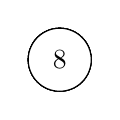
\begin{tikzpicture}[
nodes = {draw, circle, minimum size = 8mm},
edge from parent path = {(\tikzparentnode) -- (\tikzchildnode)},
sibling distance=20pt,
ed/.style = {densely dashed, shorten >= 5pt},
n/.style = {draw=none},
r/.style = {fill=white},
b/.style = {fill=gray},
edge from parent/.append style={-, shorten >= 0, shorten <= 0}]
\Tree [.\node[b]{7}; [.\node[b]{5}; [.\node[r]{1}; \edge[ed];\node[n]{}; \edge[ed];\node[n]{}; ] \edge[ed];[.\node[n]{}; ] ] [.\node[b]{10}; [.\node[r]{8}; \edge[ed];\node[n]{}; \edge[ed];\node[n]{}; ] \edge[ed];[.\node[n]{}; ] ] ]
\end{tikzpicture}
\caption{Exemplo de árvore rubro-negra. Como no resto das figuras do capítulo, os nós negros tem fundo cinza e os nós vermelhos tem fundo branco. Nas próximas figuras, o valor de cada nó não é especificado.} \label{fig:arv_bin_ex}
\end{figure}

Uma árvore rubro-negra segue as seguintes propriedades:
\begin{enumerate}
\item A raiz é preta.
\item Se um nó é vermelho, este não tem filhos vermelhos.
\item Para todo nó, todos os caminhos até links nulos de sua subárvore têm o mesmo número de nós pretos.
\end{enumerate}

Considerando apenas os nós pretos, a árvore é totalmente balanceada (propriedade 3). Como um nó vermelho não tem filhos vermelhos (propriedade 2), é possível ``juntar'' os nós vermelhos aos seus pais pretos (a raiz não é vermelha pela propriedade 1), e assim cada nó preto fica associado até~3 valores. Logo, um simples limitante superior para a altura de uma árvore rubro-negra de~$n$ nós é~$3\floor{\lg(n)}$. Se mantivermos essas propriedades a cada inserção ou remoção, e o consumo de tempo destas for proporcional à altura da árvore, então o consumo de tempo será~$\Oh(\lg n)$ para todas as operações.

\section{Implementação da persistência}

Em uma árvore rubro-negra efêmera, todo nó precisa de dois campos para seus filhos, e um valor booleano que indica se o nó é vermelho. Como já discutido, o campo booleano não precisa ser guardado de forma persistente. Como cada nó tem grau de entrada no máximo~1, no nó persistente é necessário armazenar apenas um ponteiro de volta e um ponteiro extra. O ponteiro de volta é armazenado no campo~$\V{parent}$, e é exatamente o ponteiro que aponta para o pai de um nó, o que será conveniente durante a implementação das operações. Note que, de acordo com a implementação da Seção~\ref{sec:nodecopying}, o campo~$\V{parent}$ é nulo para nós que não são ativos.

Para evitar a necessidade de replicar código muito parecido, vamos armazenar os filhos como um vetor~$\V{child}$ de~2 posições,~$u.\V{child[0]}$ é o filho esquerdo de~$u$, e~$u.\V{child[1]}$ é seu filho direito. Os campos de um nó serão:
\begin{itemize}
\item $\V{timestamp}$ --- Tempo de criação do nó.
\item $\V{copy}$ --- Próximo nó persistente (se este não é ativo).
\item $\V{child}$ --- Vetor de filhos.
\item $\V{parent}$ --- Ponteiro de volta.
\item $\V{red}$ --- Booleano que indica se o nó é vermelho.
\item $\V{extra}, \V{extraSide}, \V{extraTimestamp}$ --- Ponteiro extra, seu lado e tempo de modificação.
\end{itemize}


\end{document}
